\section*{Question 1}

\begin{wrapfigure}{r}{0.35\textwidth}
    \centering
    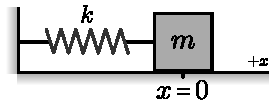
\includegraphics[scale=1]{figures/ho.pdf}
\end{wrapfigure}

A block is attached to the wall with a spring as it is shown in the figure. $k$ is the spring constant, $m$ is the mass of the body and $x=0$ is the equilibrium point of the system. It is given that the spring and all connection equipment are massless and the system is completely frictionless. We will only consider very small oscillations so that $x\ll 1$.
\begin{itemize}
    \item [\textbf{(a)}] Sketch the free-body diagrams of the block for $x>0$, $x=0$ and $x<0$. --- \textit{0.2 points}
    \item[\textbf{(b)}] Write down the equation of the motion (Newton's 2nd Law) of the block in differential equation form but do not solve it. Write the oscillation frequency $\omega_0$ in terms of $k$ and $m$. --- \textit{0.2 points}
    \item[\textbf{(c)}] By using the solution assumption $x(t)=e^{\lambda t}$ solve the equation of motion in \textbf{(b)} and write down the solution in $x(t)=Ae^{-i\omega_0 t}+Be^{i\omega_0 t}$ form, where $A$ and $B$ are some arbitrary constants. --- \textit{0.6 points}
\end{itemize}
\section*{Solution:}